\tikzstyle{input_neuron}=[circle,draw=red!50,fill=red!10,thick,minimum size=6mm]
\tikzstyle{hidden_neuron}=[circle,draw=blue!50,fill=cyan!10,thick,minimum size=6mm]
\tikzstyle{output_neuron}=[circle,draw=green!50,fill=green!10,thick,minimum size=6mm]

\tikzstyle{input}=[circle,draw=black!50,fill=black!20,thick,minimum size=6mm]

\begin{center}
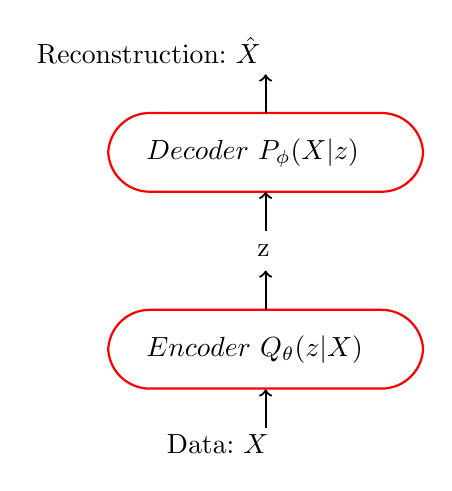
\begin{tikzpicture}

\visible<4->{
% text
\node[text width=0.007cm] at (8.40,5.75) {z};
\node[text width=0.007cm] at (7.25,3.3) {Data:~$X$};

\node[text width=0.01cm] at (6.99,4.5){$Encoder\ Q_\theta(z|X)$};

%circular rectangle
\draw[red!100,thick,solid,rounded corners=15pt] (6.5,4) rectangle (10.5,5);

%lines
\draw[thick,->] (8.5,3.5) -- (8.5,3.99);

\draw[thick,->] (8.5,5) -- (8.5,5.5);

}

\visible<5->{
	\node[text width=0.01cm] at (5.6,8.3) {Reconstruction:$\ \hat{X}$};
	\node[text width=0.01cm] at (6.99,6.99){$Decoder\ P_\phi(X|z)$};
	
	%circular rectangle
	\draw[red!100,thick,solid,rounded corners=15pt] (6.5,6.5) rectangle (10.5,7.5);
	
	%lines
	\draw[thick,->] (8.5,6) -- (8.5,6.5);
	
	\draw[thick,->] (8.5,7.5) -- (8.5,7.99);
	
}


\end{tikzpicture}
\end{center}
